\documentclass[a4paper]{article}

\usepackage[english]{babel}
\usepackage[utf8]{inputenc}
\usepackage{amsmath}
\usepackage{graphicx}
\usepackage[colorinlistoftodos]{todonotes}
\usepackage{hyperref}
\usepackage[style=numeric,backend=bibtex]{biblatex}
\usepackage{amssymb}
\usepackage{placeins}
\addbibresource{citations.bib}
\title{Project Report - NER tagging for Twitter - CMPSCI 585}

\author{Apoorva Rao Balevalachilu and Armand Halbert}

\date{\today}

\begin{document}
\maketitle

\begin{abstract}

The goal of our project is to perform Named Entity Recognition (NER) on tweets. We implemented a  feature vectors for a training and unlabeled test set of data. We then fed the feature vectors we created to CRFsuite, which then used the feature vectors to learn how to do NER on the test set.

One of our ideas for a major extension to the system involved using the Freebase API to create a powerful feature based on Freebase, a massive crowdsourced database of entities. This endeavor was not successful. However, our clustering feature using pre-created clusters from TweetNLP helped to significantly boost the performance of the system. In our paper, we demonstrate the methods we used, our results, and provide a detailed analysis of the performance of our system.  

\end{abstract}

\section{The Basics}

An example of NER is given below: \\

"Germany’s representative to the European Union’s veterinary
committee Werner Zwingman said on Wednesday consumers should ..." \\

Germany  B 
European  B
Union  I
Werner  B 
Zwingman  I
All other tokens O \\

NER is performed to identify categories such as the names of persons, organizations, locations, expressions of times, quantities, monetary values, percentages, etc.
 \\

NER can be performed for the following tasks: 
\begin{itemize}
\item Question Answering
\item Textual Entailment
\item Coreference Resolution
\item Computational Semantics
\end{itemize} 

\section{Description of Implementation}

We provide results for NER in BIO notation. Our system uses Conditional Random Fields from CRFSuite to make predictions for NER.  This model is discriminative. It does not assume that features are independent. The benefit of using a CRF is that  during labeling they are able to take future observations into account. We have used the starter code provided by Professor Brendan O' Connor and David Belanger, CRFSuite, NLTK, TweetNLP, and performed some experiments with the Freebase API.\\


We created a feature extractor that produces the following types of features. 

% mention whether you found them helpful in the end

\subsection{Lexical or wordform features}
\begin{enumerate}
\item Lowercased version of the word
\item Is in upper case?
\item Is a digit?
\item Is "retweet or RT"?
\item Is a URL?
\item Is an emoticon?
\item Is an apostrophe s?
\item Is a date?
\end{enumerate}

These were checked using regular expressions in the python code in \texttt{simple\_fe.py}

\subsection{Character Affixes}
\begin{enumerate}
\item Affixes consisting of first character
\item Affixes consisting of first two characters
\item Affixes consisting of first three characters
\item Suffixes consisting of last three characters
\item Suffixes consisting of last two characters
\item Suffixes consisting of last character
\item Begins with a hashtag i.e. \#?
\item Is a mention i.e. begins with \@?
\end{enumerate}

These were extracted using simple string manipulation code in python. 

\subsection{Shape Features}
\begin{enumerate}
\item Reduce uppercase characters - (r'[A-Z]+','A')
\item Reduce lowercase characters - (r'[a-z]+','a')
\item Reduce lowercase characters - (r'[0-9]+','0')
\item Reduce punctuations - (r'[\^A-Za-z0-9]+','\$')
\end{enumerate}

We created the shape features using regular expressions in python. 

\subsection{Positional Offset Features}
\begin{enumerate}
\item Previous word
\item Next word
\item Word before previous word
\item Word after next word
\end{enumerate}

\subsection{Major Extension - Freebase}

Freebase is a large crowdsourced database of named entities. We tried to use the \href{https://developers.google.com/freebase/v1/search}{Freebase API}. \\

Some of our sample queries are listed below: \\

\begin{itemize}
\item \href{https://www.googleapis.com/freebase/v1/search?query=robot\&indent=true\&filter=(all\%20type:animation)}{https://www.googleapis.com/freebase/v1/search?query=robot\&\\indent=true\&filter=(all\%type:animation)}
\item \href{https://www.googleapis.com/freebase/v1/search?query=robot\&indent=true\&filter=(all\%20type:people)}{https://www.googleapis.com/freebase/v1/search?query=robot\&\\indent=true\&filter=(all\%type:people)}
\item \href{https://www.googleapis.com/freebase/v1/search?query=tree\&indent=true\&filter=(all\%20type:sports)}{https://www.googleapis.com/freebase/v1/search?query=tree\&\\indent=true\&filter=(all\%type:sports)}
\item \href{https://www.googleapis.com/freebase/v1/search?query=armin\&indent=true\&filter=(all\%20type:people)}{https://www.googleapis.com/freebase/v1/search?query=armin\&\\indent=true\&filter=(all\%type:people)}

\end{itemize}

The Freebase API returns results in JSON format. The results are appended to the report.  We observed from our requests that Freebase contains entries for all kinds of things and cannot effectively identify named entities without either more comprehensive queries or a an API specifically designed for tasks in NLP. This constitutes a project in itself which demands prohibitively high effort.   \\

After our attempt, we tried to see if NER using Freebase has been tried before by anyone else. We found an answer on Stack Overflow. \\

"There is currently no equivalent project for named entity recognition in Freebase. However, Freebase has links to DBpedia on sameAs.org so you can use DBpedia spotlight and then resolve the IDs back to Freebase and that data is also available in the Freebase RDF dumps. \\

If you're looking for a coding project in this area, I think it should be possible to adapt the DBpedia Spotlight code so that you can train its models using Freebase data. The main benefit of this would be that Freebase covers a wider range of entities than DBpedia so you'd get better recall. Also, you may be able to exploit other data in Freebase like "notable types" to get better precision as well.\\

You should be able to get a good set of "surface forms" of the entity by looking at the /type/object/name and /common/topic/alias properties in Freebase. Any Freebase entity that corresponds to a Wikpedia page will have one or more /type/object/key values in the /wikipedia/en namespace. These correspond to the Wikipedia page names (and redirects) which will allow you to parse through the Wikipedia XML dumps and identify which links on the page correspond to Freebase topics. The Freebase key encoding scheme is described here. \\

You might also be interested in OpenCalais and AlchemyAPI which provide named entity recognition as a service and provide Freebase IDs in their API responses."\cite{so}\\

We hope to be able to use this information to enhance future versions of our NER Tagger. We decided not to incorporate a feature that uses the Freebase API this time. Our code is attached. \\


\subsection{Major Extension - Part-Of-Speech Tagger}

We used an external POS tagger(NLTK) to generate features.\cite{loper2002nltk} Named entities are closely related to their part of speech. The most common POS to be a named entity are nouns. Verbs, pronouns, and adjectives can be named entities, but are far less common. \\

We implemented POS tagging using "Natural Language Toolkit" for Python. This POS Tagger is not specifically designed to be able to accurately provide POS tags for tweets. The peculiar characteristics of tweets make them unlike other forms of text. For example, twitter has it's own jargon and modifications to english grammar. The performance of our system could possibly be enhanced by using a tool is specifically designed for this purpose, like the tweetNLP POS tagger. \cite{gimpel2011part}\\

We complemented the POS tag feature by adding a positional offset variation feature for POS tags which effectively helps the CRFSuite consider a POS tag context. \\

\newpage

\subsection{Major Extension - Brown Clustering Feature}

We then implemented a feature for Brown Cluster IDs. Many packages which perform clustering are available on GitHub. We considered the following two options: \\

\href{https://github.com/mheilman/tan-clustering.git}{Brown Clustering in Python by Michael Heilman}.\\

\href{https://github.com/percyliang/brown-cluster.git}{Percy Liang's C++ implementation of Brown Clustering} produced by an unsupervised Hidden Markov Model.\\

We chose to go with the second option indirectly by performing a lookup on the results of a large clustering experiment performed over tweets from 2008 to 2012. 56,345,753 tweets in total. In our opinion, this was the wiser choice because creating our own clusters by implementing brown clustering on our training dataset and the 1 million tweets unlabeled data set shared in the class could not be as extensive as the clustering dataset coverage we'd get by using a larger resource. \cite{50mpaths} A drawback with this approach is that the 1 million unlabeled tweets shared in class possibly have newer words that entered the vocabulary during the period from 2012 to 2014. However, since this is just two years, we can safely assume, without much loss to model accuracy, that such "new" words aren't too numerous in the test set.\cite{gimpel2011part}. The ablation tests we conducted show an improvement upon adding this feature. The results are presented in a tabular manner in the Analysis section. Clustering done on any other dataset, apart from tweets, would not help us as much.  

\subsection{Simple Observations}

We created a feature for the word itself. \\

We found that checking word capitalization is valuable for Named Entity Recognition.The problem is that Twitter users do not adhere to english capitalization rules. \\

The affixes features we created were useful for NER tagging because we found that many of the rules allowed a token to be tagged 100\% accurately. For example, emoticons, hashtags and mentions are featured as "never an entity". We could then pass that feature to CRFsuite, which would quickly learn that those features would always be tagged O. This increased the precision of our classifier greatly, since we were far less likely to classify certain things as named entities. Initially, we found hashtags and mentions would never be named entities. We later expanded this list to include emoticons, punctuation symbols, dates and urls. \\

We also found that certain suffixes indicated a word was not a named entity. For example, consider verb modifiers . Words ending in -er or -ing are generally verbs, which are much less likely to be named entities than nouns. This helped remove false positives from our system. Since we were not identifying named entities, however, it did not improve our recall.  \\

Another feature of our system was to simplify word shape. Shape allowed us to turn capitalization into a simple common feature.  Most named entities tended to start with capital letter, followed by a word. This feature allowed us to generate simple features, such as feature "Aa" for a word starting with a capital letter, and feature "a" for words that did not start with a capital letter, or were entirely lowercase. We incorporated "\$" for punctuations and "0" for numbers. This allows CRF suite to decide how to weight variations, rather than us manually developing complex regular expressions as features to gain the equivalent word-shape feature. \\

We incorporated positional offset features for previous words, next words, previous POS tag, next POS tag. Taken along with the word shape feature, this helped increase system performance in terms of F-score proportionately from 0.08 to 0.23. \\

The brown clustering feature was the most powerful feature of all. A detailed analysis is provided in the following sections. 


\section{Results}
We achieved an F-score of \texttt{0.23644} at the end of the Kaggle competition, but improved our system significantly after that. \\

At the time of the competition, we did not implement enough context features. We also did not have a clustering feature, and did not use regularization before the close of the competition. \\

At present, our scores using the train plus dev set for training and test set for testing are: \\

\begin{enumerate}

\item LBFGS with L2-regularization of c2=0.00001 \\
\texttt{Span-level NER evaluation}\\
\texttt{F = 0.5217,  Prec = 0.6963 (674/968),  Rec = 0.4171 (674/1616)}\\
\texttt{(3336 sentences, 46714 tokens, 1616 gold spans, 968 predicted spans)}\\

\item SGD with L2-regularization of c2 = 0.01 \\
\texttt{Span-level NER evaluation}\\
\texttt{F = 0.5158,  Prec = 0.6961 (662/951),  Rec = 0.4097 (662/1616)}\\
\texttt{(3336 sentences, 46714 tokens, 1616 gold spans, 951 predicted spans)}\\

\item Averaged Perceptron \\
\texttt{Span-level NER evaluation}\\
\texttt{F = 0.5265,  Prec = 0.6357 (726/1142),  Rec = 0.4493 (726/1616)}\\
\texttt{(3336 sentences, 46714 tokens, 1616 gold spans, 1142 predicted spans)}\\

\item Passive Aggressive \\
\texttt{Span-level NER evaluation}\\
\texttt{F = 0.5340,  Prec = 0.6676 (719/1077),  Rec = 0.4449 (719/1616)}\\
\texttt{(3336 sentences, 46714 tokens, 1616 gold spans, 1077 predicted spans)}\\

\item Adaptive Regularization of Weights \\
\texttt{Span-level NER evaluation}\\
\texttt{F = 0.4150,  Prec = 0.4581 (613/1338),  Rec = 0.3793 (613/1616)}\\
\texttt{(3336 sentences, 46714 tokens, 1616 gold spans, 1338 predicted spans)}\\

\end{enumerate}
%write about shape features, context features i.e. positional offset features

\section{Analysis / Exploration}

\subsection{Regularization}

We explore different hyperparameter settings in conjunction with two of the algorithm choices provided by CRFSuite. We graph L2 regularizer strength (which is called c2 in CRFSuite) against test set performance. 

{\centering
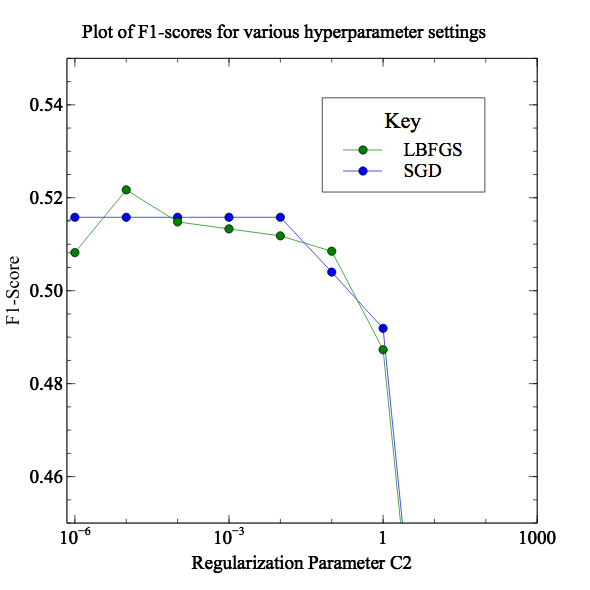
\includegraphics[width=0.90\textwidth]{regularization-graph.png}
} \\

The graphs indicate optimal values for c2 in both cases. 

To summarize, we have shown clearly how the system performs using two Machine Learning Algorithms, namely:  
\begin {enumerate}
\item LBFGS with L2 Regularization
\item SGD with L2 Regularization
\end {enumerate}


\subsection{Learning Curve}
%Graph a learning curve: see how devset performance improves when you train with more data (or how it worsens with smaller subsamples of the training data). A learning curve has the y-axis as devset performance, and the x-axis as training set size. If it hasn't flattened out yet, it may be useful to annotate more data. (Doing just a learning curve on the original training data is good, but it's not enough to count as a full analysis component.) To count for credit, make at least 1 graph similar to the Miller et al. 2004 graph (or like the Koo et al. 2008 table) that was in the 11/18 lecture.

We plotted a learning curve using fractions of the data (without shuffling). \\

\begin {enumerate}
\item Y Axis - Test Set Performance in terms of F-score, precision and recall. 
\item X Axis - Training Set Fraction. 
\end {enumerate}


We have 20378 entries in our train.feats file. We split this into four parts 5094 entries each. We will not use the single entry in a fifth file in order to prevent having skewed results. \\

{
\centering
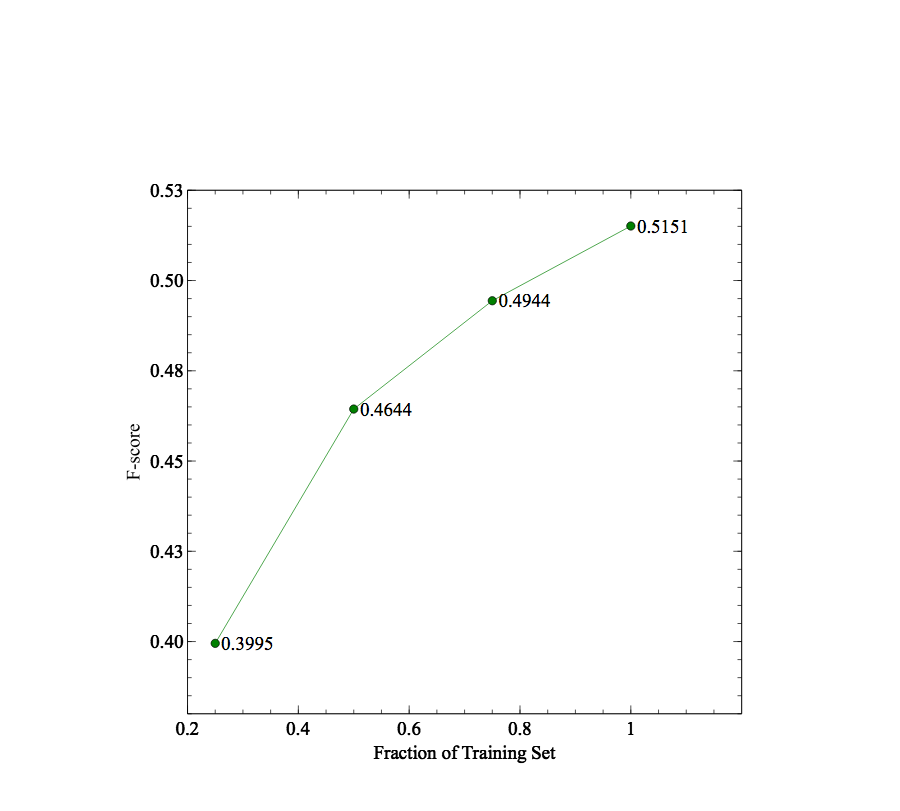
\includegraphics[width=0.90\textwidth,trim=2cm 1cm 2cm 2cm,clip]{f-score.png}
}


{
\centering
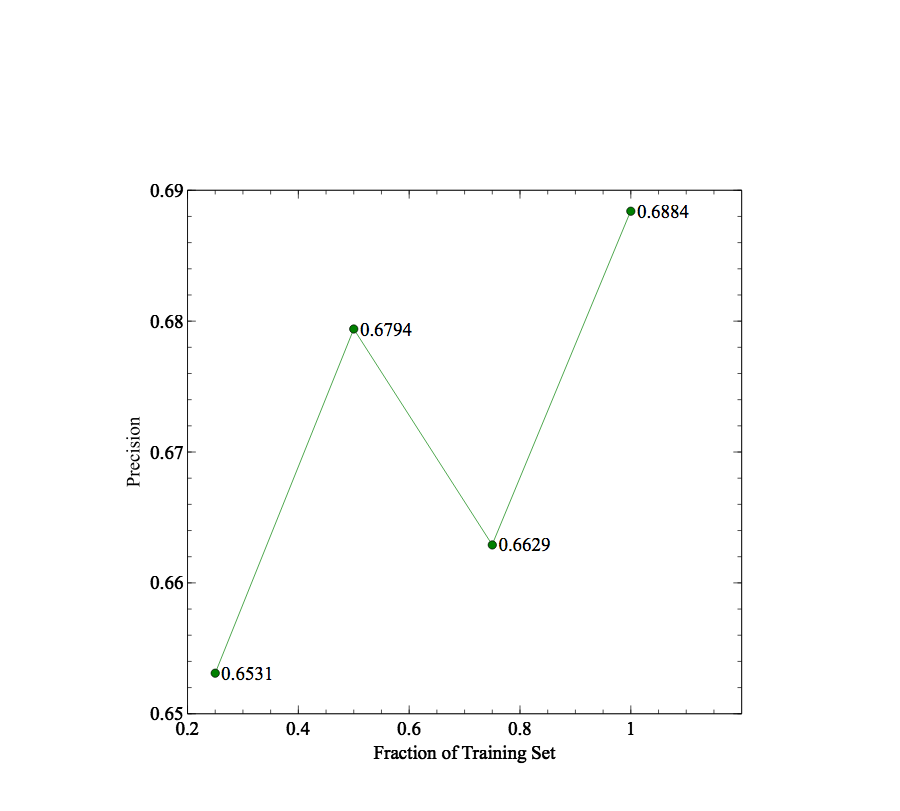
\includegraphics[width=0.90\textwidth,trim=2cm 1cm 2cm 2cm,clip]{frac-prec.png}
}

{
\centering
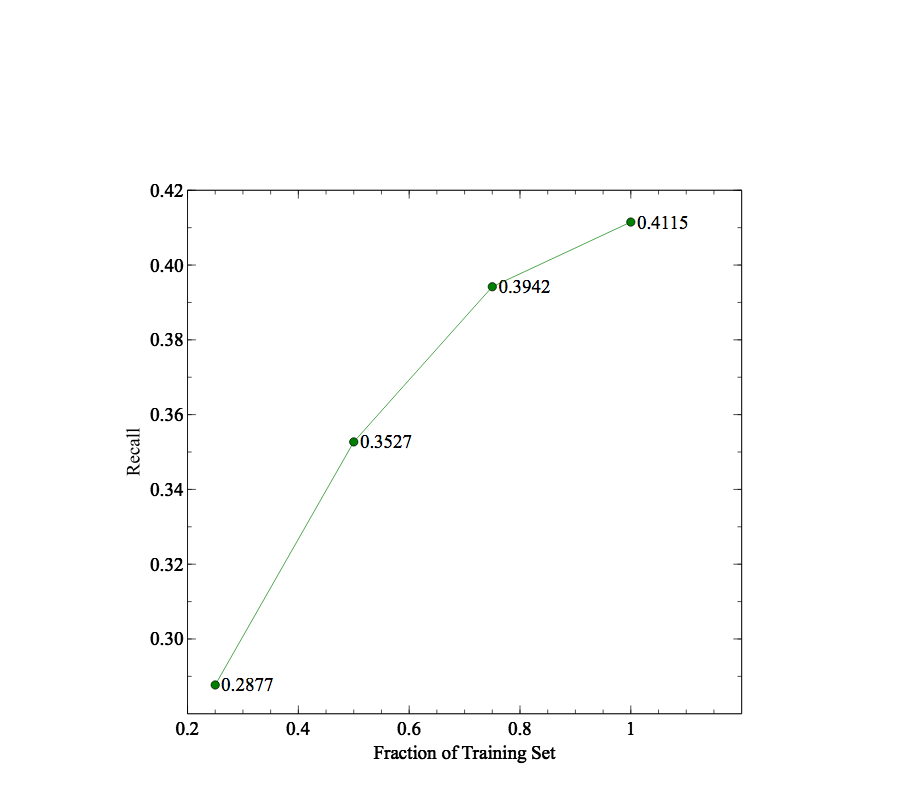
\includegraphics[width=0.90\textwidth,trim=2cm 1cm 2cm 2cm,clip]{recall.png}
}



We can conclude by looking at this graph that it will be useful to annotate more data because the curve has not yet flattened out. 


\subsection{Ablation testing}

For ablation testing we can remove classes of features from the final model to see how much the performance goes down or take a base system and add classes of features to see how much performance improves. We go with the latter option and illustrate our results with the table below. 

\begin{table}[h]
\begin{tabular}{|l|c|c|c|c|c|c|}
\cline{1-7}
F-Score & Lexical/  & Character & Shape & Positional & POS & Clustering \\ 
& Wordform & Affix & & Offset & Tag & \\ 
\cline{1-7}
0.0355 & \checkmark & & & & & \\\hline
0.0826 & \checkmark & \checkmark & & & & \\\hline
0.2364 & \checkmark & \checkmark & \checkmark & \checkmark & & \\\hline
0.3821 & \checkmark & \checkmark & \checkmark & \checkmark & \checkmark & \\ \hline
0.5118 & \checkmark & \checkmark & \checkmark & \checkmark & \checkmark & \checkmark\\\hline

\end{tabular}
\end{table}

\section{Discussion and Future Work}

One of our attempts at the beginning that did not work out was adding on extra data. We initially added on all the data provided in the git repository by Ritter et al., but found that it would overfit and take forever to run. \\

CRFSuite uses linear chain CRFs. We could explore the option of using higher order CRFs. The Factorie package offers options to perform such experiments in NER and other tasks in NLP.  Not all classification algorithms are created equal\cite{springer1}, it is entirely possible that using a more innovative ML algorithm than the ones provided with CRFSuite yield better results. \\

We could also use resources like language dictionaries and Freebase during the evaluation stage. \\

Another idea is to learn word embeddings from unlabeled data. This helps dealing with very large and sparse vectors that incorporate context features. \\

Being able to work on more specialized systems can help us gain better prediction results. There is no point in reinventing the wheel. One option would be the Stanford Named Entity Recognition system. MITIE also offers Named Entity Recognition systems, and also offers python bindings. However, we would prefer to use the source code as inspiration, to add more features like the ones mentioned above and suggested in class to obtain better results. \\


\printbibliography
\end{document}